\section{xv6的系统结构}

SMP是Symmetric Multi Processing的简称,意为对称多处理计算机系统,内有许多紧耦合多处理器,这种系统的最大特点就是共享所有资源。在SMP架构中,每个处理器在功 能上都是对称、等价的。每个处理器有独自的中断处理控制器(硬件)。 内存在所有处理器之间共享。因此处理器可以通过共享的内存区域进行通讯。Xv6就是一个SMP操作系统,可以有多个cpu公共工作.

xv6基于典型的UNIX操作系统设计思路。简单地说,xv6是一种能区分内核态和用户态,基于扁平内存管理的层次型单体内核,应用程序和操作系统是处于不同的特权状态和地址空间。代表应用程序的用户态进程运行在CPU的用户态(又称非特权模式,用户模式),无法直接访问系统硬件和操作系统中的系统数据,而操作系统运行在CPU的核心态(又称特权模式,内核模式),可以访问系统硬件和核心数据。下面给出一个xv6系统结构是示意图

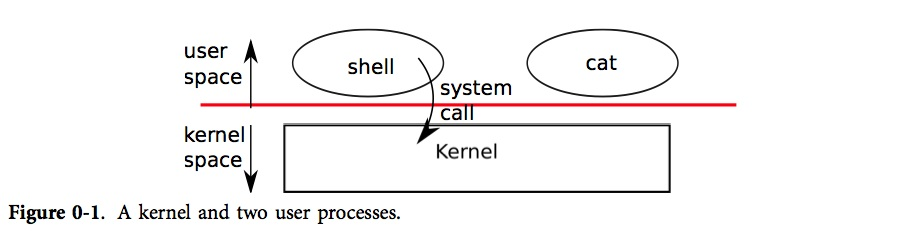
\includegraphics[width=6in]{figures/struct/fig1.png}

下面分别从系统调用接口、进程/线程管理、内存管理、文件系统、I/O管理等几个方面进行总体分析。

进程通过系统调用使用内核服务。系统调用是应用程序访问操作系统的接口。在系统调用接口上,通用操作系统与基于此操作系统的应用程序处于两个不同的CPU特权态,操作系统处于核心态,而应用程序处于用户态。在核心态可以执行CPU特权指令,而用户态无法执行特权指令,且只能通过特定的指令或中断来访问操作系统提供的各种功能。这在一定程度上保证了系统整体的安全,避免应用程序对操作系统可能的破坏。内核使用了 CPU 的硬件保护机制来保证用户进程只能访问自己的内存空间。内核拥有实现保护机制所需的硬件权限(hardware privileges),而用户程序没有这些权限。当一个用户程序进行一次系统调用时,硬件会提升特权级并且开始执行一些内核中预定义的功能。内核提供的一系列系统调用就是用户程序可见的操作系统接口,xv6 内核提供了 Unix 传统系统调用的一部分,它们是:

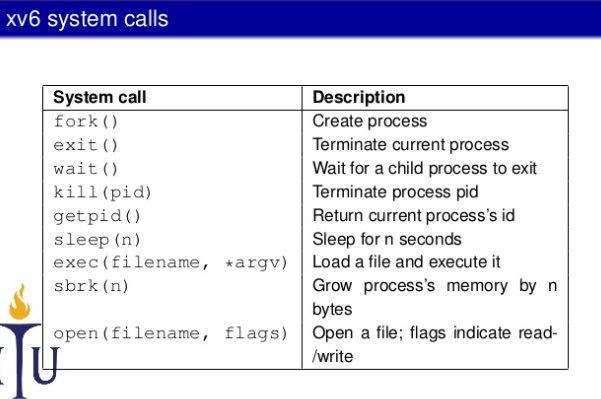
\includegraphics[width=6in]{figures/struct/fig2.png}

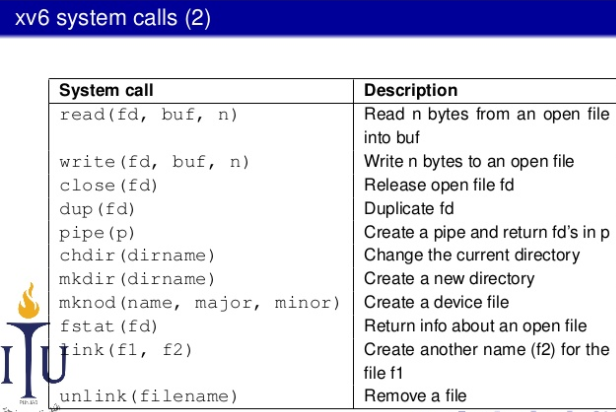
\includegraphics[width=6in]{figures/struct/fig3.png}

在内存管理方面,通用操作系统采用了虚拟内存管理方式,这样可以让内存需求超过实际物理内存的进程/线程能够执行,其主要思想是把重要和常用的数据和执行代码放在物理内存中,把不常用的数据和执行代码放到二级存储(这里主要指的是硬盘等可在掉电后保存数据的存储介质),随时根据系统执行情况替换放在内存中的数据和代码。而且通过虚存管理可以实现对不同内存区域的保护,不同进程之间,或者应用程序和操作系统之间的地址空间相对隔离。这样一般情况下不同进程的地址空间不能直接访问,且应用程序不能直接访问内核地址空间。所以一个与错误的应用程序不会导致系统的崩溃,从而增加了系统的可靠性。xv6操作系统没有采用虚拟内存管理,而是采用了简单的基于X86段模式的单一地址空间管理方式。在内存分配和释放的管理上,xv6相对实现得比较简单,采用基于可变分区分配的首次适配算法,容易产生内存碎片。

在进程/线程管理方面,当前通用操作系统结合虚存管理,采用进程和线程结合的管理方式。进程代表了一个程序执行的过程以及其所占用的计算机资源(包括CPU、内存、文件等),进程的执行流可用线程来表示。操作系统的调度单位可以是进程或线程。一个进程可以包含多个线程,属于同一进程的多个线程共享进程管理的资源,比如属于同一进程的多个线程共享进程所管理的内存,这样这些线程可以直接访问属于进程的全局地址空间。 xv6操作系统实现了一个基于进程(没有实现线程)的简单进程管理机制。

在文件系统管理方面,当前通用操作系统结合虚存管理,实现了多种复杂、高效且可靠的文件系统,且建立了一个统一的虚拟文件系统层,屏蔽不同文件系统的差异,对上层提供统一的接口。且与用户管理和进程管理结合,可实现安全管理,保证对文件的安全访问。xv6操作系统实现了一个相对简单的基于inode索引方式的文件系统。

在I/O管理方面,xv6操作系统与通用操作系统(特别是类UNIX操作系统)差别不是特别大,都把设备“看成”是一种特殊的设备文件,有设备号,用文件的访问接口来进行打开、关闭、读、写和控制等操作。在灵活性方面,xv6驱动程序不能象通用操作系统那样根据硬件情况动态加载,而是在编译时候就静态确定的。
